\section{Simulación}\label{sec:simulation}

Para comprobar el sistema de control se definió el sistema no-lineal en \Matlab, se obtuvo el sistema lineal sobre un punto de operación tomando el jacobiano del sistema de ecuaciones diferenciales para controlar el sistema, y finalmente se integró el sistema no lineal en el tiempo retroalimentado con el sistema de control.

Se investigó la respuesta del vehículo ante perturbaciones Delta-Dirac de orientación.

\subsection{Sistema no-lineal}

El sistema~\eqref{eq:ssDiffVariables3D} describió la dinámica no-lineal del vehículo con 16 ecuaciones. Estas pudieron ser integradas mediante un método numérico para ecuaciones diferenciales ordinarias multivariables no-autónomas. El requerimiento no-autónomo surgió de la necesidad de incorporar el vector $\Cu$ a la integración, el cual incluyó las actuaciones en base a lo que leyeron los sensores. 

\medskip

Para satisfacer el requerimiento no-autónomo se tuvo que implementar un método numérico basado en Runge-Kutta orden 4. El método fue probado y contrastado con soluciones analíticas conocidas.

\subsection{Sistema de control}

Se optó por controlar mediante el controlador \gls{lqr} debido a la simplicidad de implementación y adaptabilidad para problemas de variables de estado. Como se mencionó anteriormente, se obtuvo el jacobiano del sistema \eqref{eq:ssDiffVariables3D} alrededor del punto de operación. Esta se denominó la matriz del sistema $\MA$. La matriz $\MB$ formó parte del jacobiano del sistema pero diferenciado respecto $\Cu$. Finalmente, $\MC$ resultó la combinación lineal de las mediciones de los sensores (ver sección \ref{sec:model2d} para entender el proceso). 

Se modelaron las siguientes imperfecciones en el sistema:

\begin{itemize}
    \item Delay en medición/actuación
    \item Desalineación de sensores (acelerómetro y giroscopio)
    \item Resolución mínima de actuación del gimbal según lo visto en la sección~\ref{ssec:servoSeleccion}
\end{itemize}

La matriz costo del controlador LQR asociada al equilibrio se construyó asignando los siguientes valores a la diagonal: 5 a las posiciones globales, 1 a las velocidades, $1\times10^{-3}$ a la velocidad del rotor del EDF, $1\times10^{-4}$ a la velocidad angular en pitch y yaw del vehículo, y $1\times10^{-5}$ a las variables restantes (actuadores, ángulos de Euler y velocidad angular en roll).

\medskip

La matriz costo asociada a los actuadores es diagonal con los siguientes valores: 1000 a actuadores de pitch y yaw del gimbal, $1\times10^{-5}$ al actuador de roll, y $1\times10^{-6}$ al control velocidad del rotor del EDF.


\subsection{Resultados de simulación}

Los ejes $x$ corresponden al tiempo en segundos. El vehículo comenzó con una perturbación Delta-Dirac en la orientación del ángulo de euler $\phi$ y a una altura de 1m (en $z$) con velocidad nula. Los gráficos describen la evolución de las variables de estado en el tiempo luego de la perturbación. Durante esta simulación el control estaba activo y, como se puede ver en los gráficos de posición, previnió que el vehículo descienda más de 2 metros de altura. También pudo recuperar su estado de equilibrio con todas las variables de estado de actitud acercandosé asimptoticamente a cero transcurrido 6 segundos desde la perturbación.

\begin{figure}[!ht]
    \centering
    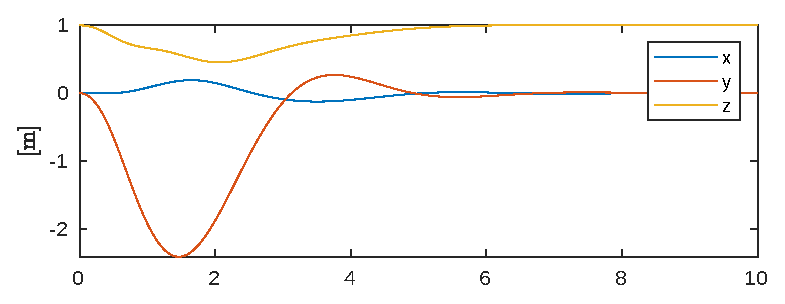
\includegraphics[width=0.8\linewidth]{fig/pos_edf}
    \caption{Posición del vehículo}
    \label{fig:pos_edf}
\end{figure}

\begin{figure}[!ht]
    \centering
    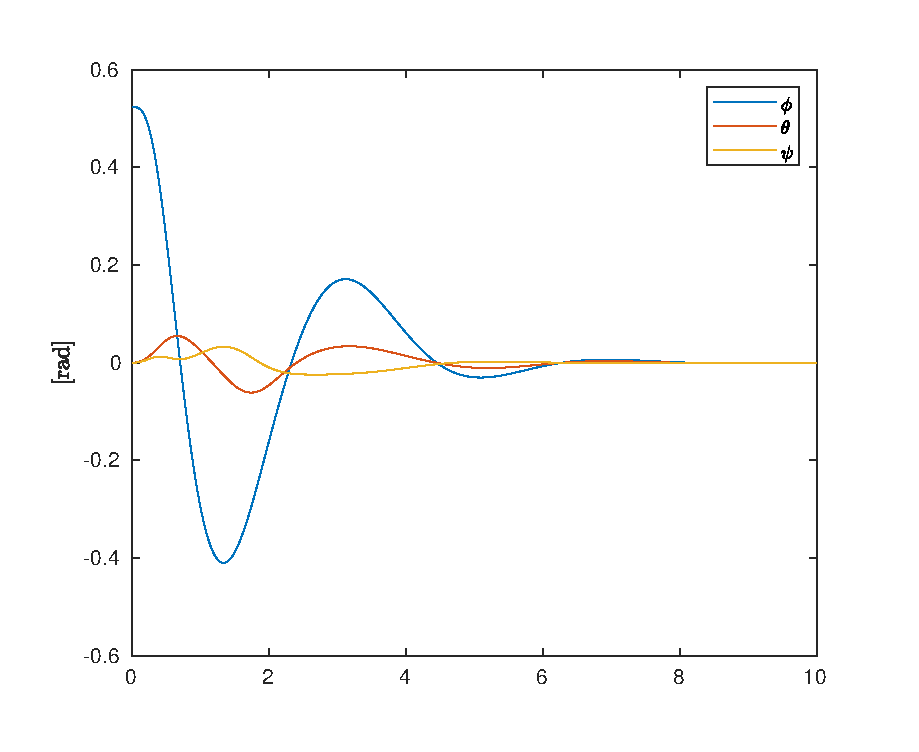
\includegraphics[width=0.6\linewidth]{fig/eulerang_edf}
    \caption{Ángulos de euler. Note que solo hubo perturbación inicial en $\phi$ sin embargo la actuación del gimbal ($\alpha$) generó una perturbación interna en $\theta$ por el efecto giroscópico.}
    \label{fig:eulerang_edf}
\end{figure}

\begin{figure}[!ht]
    \centering
    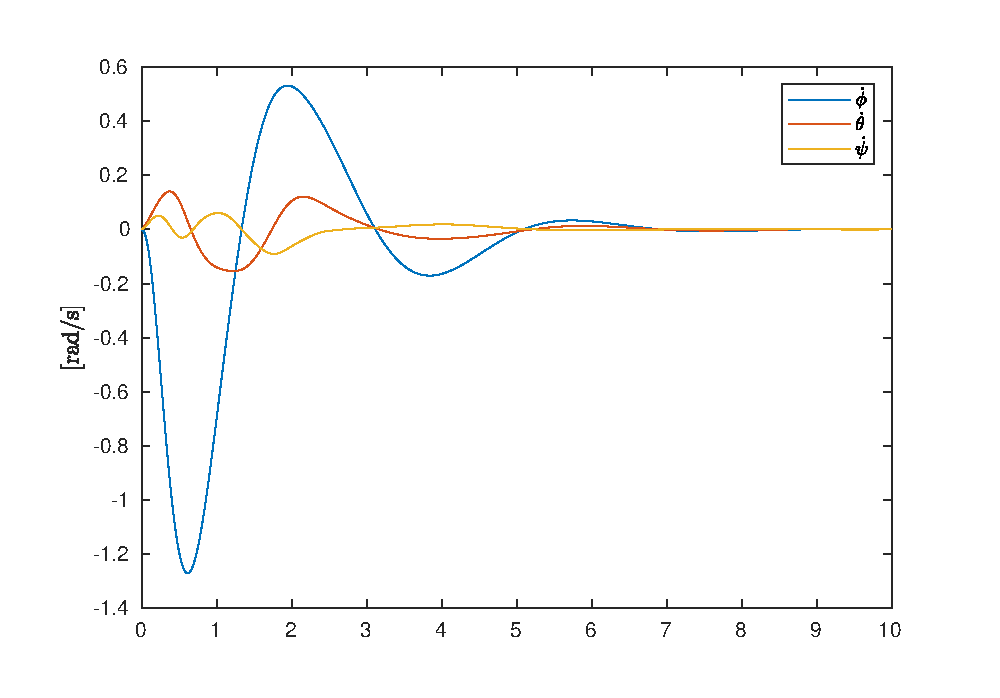
\includegraphics[width=0.6\linewidth]{fig/angvel_edf.eps}
    \caption{Velocidad angular del vehículo}
    \label{fig:angvel_edf.eps}
\end{figure}

\begin{figure}[!ht]
    \centering
    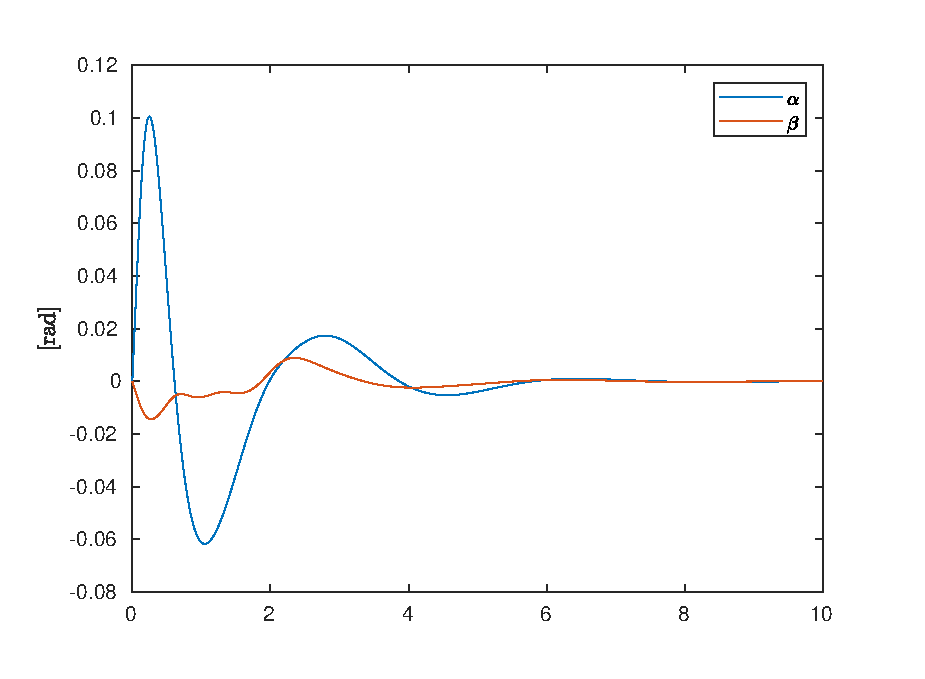
\includegraphics[width=0.6\linewidth]{fig/actuator_edf}
    \caption{Actuación angular del gimbal.}
    \label{fig:actuator_edf}
\end{figure}

\begin{figure}[!ht]
    \centering
    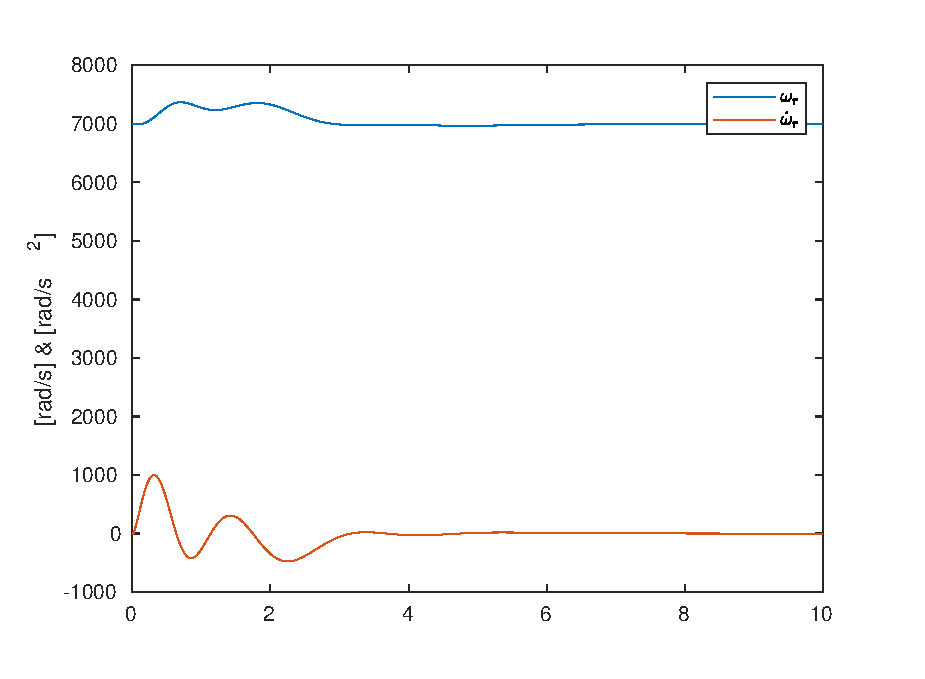
\includegraphics[width=0.6\linewidth]{fig/rotor_edf}
    \caption{Velocidad y aceleración angular del rotor.}
    \label{fig:rotor_edf}
\end{figure}



